\section{Régulateur PID}

Afin de réaliser la fonction de régulation PID avec un FeedForward, il est nécessaire de d'abord
définir les fonctions Lead-Lag (pour la partie FeedForward) et IMC Tuning (pour le calcul des constantes $K_c$, $T_i$ et $T_d$).

\subsection{FeedForward}

\begin{figure}[h]
    \centering
    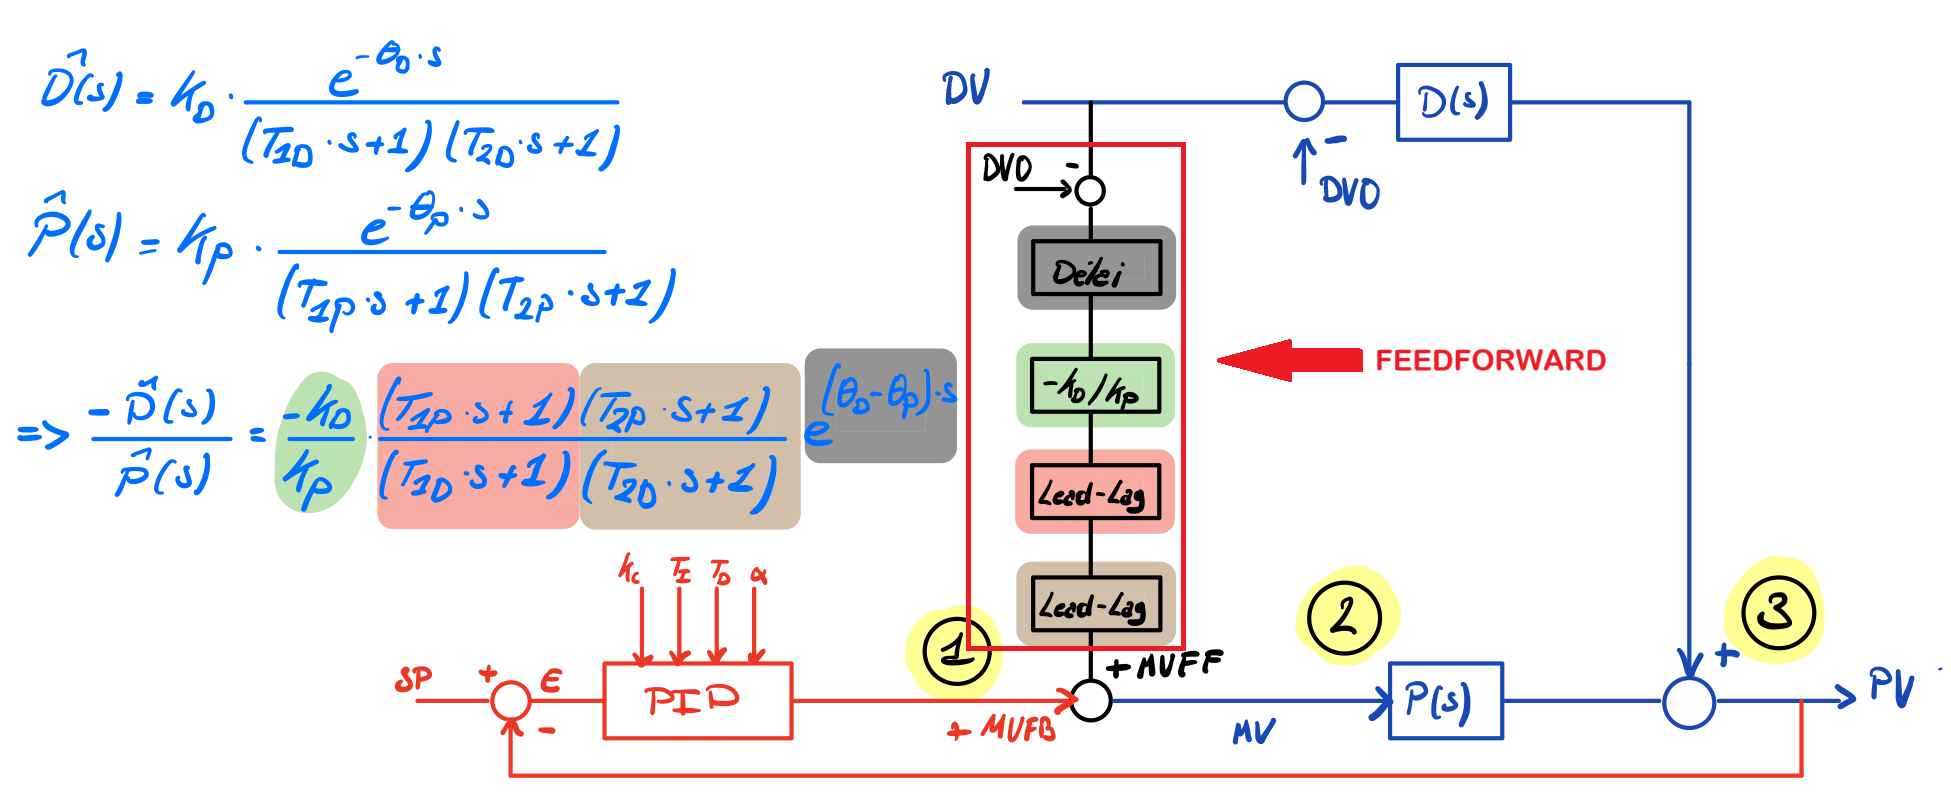
\includegraphics[width=\textwidth]{figures/schemaFF.png}
    \caption{Schema du régulateur PID avec fonction de FeedForward}
	\label{fig:schemaFF}
\end{figure}

La fonction de FeedForward est conçue pour anticiper et compenser l'impact des perturbations ($DV$) sur la variable du processus ($PV$), 
avant que ces dernières n'affectent le système.
\\Le fonctionnement du FeedForward peut être décrit de manière mathématique comme suit : 
\begin{itemize}
	\item 
	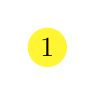
\begin{tikzpicture}
		\fill[fill=yellow!80!] (0,0) circle [radius=0.25cm];
		\node at (0,0) {1};
	\end{tikzpicture} Premièrement, la valeur manipulée en sortie du PID, $MV_{FB}$, est ajustée par une valeur $MV_{FF}$, calculée pour compenser directement la perturbation :
	\[MV_{FF} = K_{FF}\cdot\frac{(T_{1P}s + 1)(T_{2P}s + 1)}{(T_{1D}s + 1)(T_{2D}s + 1)}\cdot e^{-\theta_{FF}}\,DV = \frac{\hat{D}(s)}{\hat{P}(s)}\,DV\]
	avec : 
	\[K_{FF} = \frac{K_D}{K_P},\,\theta_{FF} = |\theta_D - \theta_P|\]
	\item 
	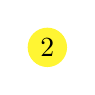
\begin{tikzpicture}
		\fill[fill=yellow!80!] (0,0) circle [radius=0.25cm];
		\node at (0,0) {2};
	\end{tikzpicture}Ensuite, après le n\oe{}ud $MV = MV_{FB} + MV_{FF}$, on obtient : 
	\[P(s)\cdot MV \approx P(s)\cdot MV_{FB} - \hat{D}(s)\]
	\item
	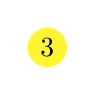
\begin{tikzpicture}
		\fill[fill=yellow!80!] (0,0) circle [radius=0.25cm];
		\node at (0,0) {3};
	\end{tikzpicture} Pour enfin arriver au n\oe{}ud final où l'on additionne la dynamique de la perturbation à celle du processus : 
	\[P(s)\cdot MV_{FB} - \hat{D}(s) + D(s) \approx P(s)\cdot MV_{FB} = PV\]
\end{itemize}
\subsubsection{Délai}

La $1^{ère}$ étape dans la réalisation de la fonction du ``FeedForward'' est de récupérer la perturbation $DV$, de la ramener au point de fonctionnement et de lui appliquer un délai $\theta_{FF} = |\theta_D-\theta_P|$ qui provient du rapport entre la dynamique de la perturbation
$\hat{D}(s)$ et du processus $\hat{P}(s)$.
Pour se faire, on utilisera la fonction \texttt{Delay\_RT} sur le signal $DV$ recentré via : 
\begin{python*}
	Delay_RT(self.DV - self.DV0*np.ones_like(self.DV), # On centre DV sur le point de fonctionnement
		max(self.theta_ODV_SOPDT-self.theta_OMV_SOPDT, 0), # Calcul du délai 
		self.Ts, 
		self.MVFF_Delay)
\end{python*}

\subsubsection{Gain et Lead-Lag}
Une fois que le délai et la translation appliqués, il faut maintenant passer au gain et au premier Lead-Lag.
\\Le gain est simplement le rapport du gain de la fonction de transfert décrivant la dynamique de perturbation et celle décrivant la dynamique de processus $K_{FF} = \frac{K_D}{K_P}$ (la raison du signe négatif sera expliquée plus tard dans le rapport).
\\Le premier Lead-Lag dont $T_{Lead} = T_{1D}$ et $T_{Lag} = T_{1P}$ couplé au gain et au délai permet d'obtenir la fonction de transfert : 
\[K_{FF}\cdot\frac{T_{1D}s + 1}{T_{1P}s + 1} \cdot e^{\theta_{FF}}\]
Pour se faire, on utilise la fonction \texttt{LL\_RT} sur le signal $DV$ retardé et centré ($MV\_Delay$) via : 
\begin{python*}
	LL_RT(self.MVFF_Delay, 
	-self.Kp_ODV_SOPDT/self.Kp_OMV_SOPDT, # gain
	self.T1_OMV_SOPDT, 
	self.T1_ODV_SOPDT, 
	self.Ts, 
	self.MVFF_LL1)
\end{python*}




